%%%%%%%%%%%%%%%%%%%%  DATA BREACH %%%%%%%%%%%%%%%%%%%%%%%%
\newpage
\subsection{Data Breach}
\subsubsection{Lower Bound Computation}
\[
\begin{bmatrix}
\mathbf{x}_{\text{American Samoa}}^{(\text{count})}\\
\mathbf{x}_{\text{American Samoa}}^{(\text{dollars})}
\end{bmatrix}
=
\begin{bmatrix}
0 & \cdots & 0 & \cdots & 0\\
\$0 & \cdots & \$0 & \cdots & \$0
\end{bmatrix}.
\]
% Columns represent years 2016, \cdots, 2017, \cdots, 2022 for American Samoa Data Breach.
% Raw counts: 2016=0, 2017=0, 2022=0.  Raw dollars: 2016=\$0, 2017=\$0, 2022=\$0.
\[
\begin{bmatrix}
\mathbf{x}_{\text{American Samoa}}^{(\text{count scaled to sample population})}\\
\mathbf{x}_{\text{American Samoa}}^{(\text{dollars scaled to sample population})}
\end{bmatrix}
=
\begin{bmatrix}
0 & \cdots & 0 & \cdots & 0\\
\$0 & \cdots & \$0 & \cdots & \$0
\end{bmatrix}.
\]
% Per-capita scaled to Chattanooga population: 2016=0, 2017=0, 2022=0 victims; dollars: all \$0.
  \[
\bar{X}_{\text{American Samoa}}^{(m)}
= \frac{1}{N}\sum_{i=1}^{N} X_{\text{American Samoa},i}^{(m)},
\]
\\
\[
\qquad
m \in \{\text{scaled count},\text{scaled dollars}\}
\]
\[
\begin{bmatrix}
\bar{X}_{\text{American Samoa}}^{(\text{scaled count})}\\
\bar{X}_{\text{American Samoa}}^{(\text{scaled dollars})}
\end{bmatrix}
=
\begin{bmatrix}
0.43\\
\$166{,}890
\end{bmatrix}.
\]
\subsubsection{Upper Bound Computation}
\[
\begin{bmatrix}
\mathbf{x}_{\text{California}}^{(\text{count})}\\
\mathbf{x}_{\text{California}}^{(\text{dollars})}
\end{bmatrix}
=
\begin{bmatrix}
568 & \cdots & 632 & \cdots & 381\\
\$9{,}769{,}361 & \cdots & \$7{,}805{,}797 & \cdots & \$1
\end{bmatrix}.
\]
% Columns represent years 2016, \cdots, 2017, \cdots, 2022 for California Data Breach.
\[
\begin{bmatrix}
\mathbf{x}_{\text{California}}^{(\text{count scaled to sample population})}\\
\mathbf{x}_{\text{California}}^{(\text{dollars scaled to sample population})}
\end{bmatrix}
=
\begin{bmatrix}
2 & \cdots & 2 & \cdots & 2\\
\$34{,}399 & \cdots & \$24{,}702 & \cdots & \$121{,}084
\end{bmatrix}.
\]
\[
\bar{X}_{\text{California}}^{(m)}
= \frac{1}{N}\sum_{i=1}^{N} X_{\text{California},i}^{(m)},
\]
\\
\[
\qquad
m \in \{\text{scaled count},\text{scaled dollars}\}
\]
\[
\begin{bmatrix}
\bar{X}_{\text{California}}^{(\text{scaled count})}\\
\bar{X}_{\text{California}}^{(\text{scaled dollars})}
\end{bmatrix}
=
\begin{bmatrix}
1.26\\
\$44{,}615
\end{bmatrix}.
\]
\subsubsection{Monte Carlo Simulations for Likelihood and Impact}
\begin{figure}[H]
  \centering
  \rotatebox{0}{\scalebox{1}{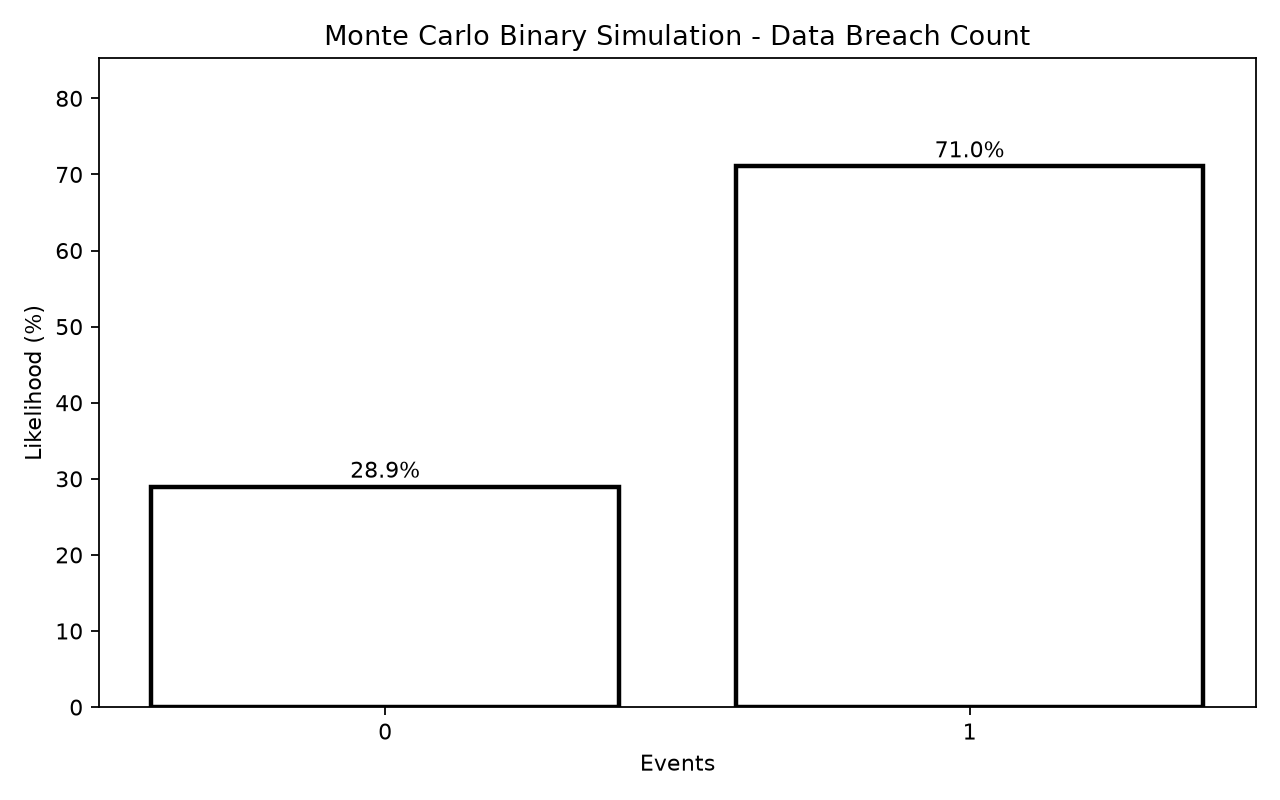
\includegraphics[scale=0.25]{figures/binary_dataBreach_count.png}}}
  \caption{We ran a\index{Monte Carlo simulation} Monte Carlo simulation of 10,000 iterations with a binary distribution to spread random instances between upper and lower bounds taken from the means of seven year samples. We bounded between 0 and 1 possible \index{data breach}data breach events over a year.\protect\endnote{\index{sample} Sample size was set equivalent to the City of\index{Chattanooga} Chattanooga to determine the per capita rates for each year over data from \index{American Samoa} American Samoa and\index{California} California.  The means of those rates were used to set upper and lower bounds with \index{American Samoa} American Samoa and\index{California} California representing low and high \index{cybercrime} cybercrime counts respectively.}
  \protect\endnote{Monte Carlo Modeling Toolkit authored by Derek E. Brink, CISSP, \url{www.linkedin.com/in/derekbrink}. March 2023.}
  }
  \label{fig:screenshot-montecarlo-databreach-count-binary}
\end{figure}
When we computed the upper and lower bounds, we recognized that a normal distribution would not fit well for forecasting likelihood.  We took the mean of the sample from American Samoa for the lower bound (0); we took the mean from the sample from California for the upper bound (1); we had a separation of 1 unit.  Therefore, we switched to a binary model with 2 possible outcomes.
\begin{table}[H]
  \centering
  \caption{Monte Carlo Binary Simulation Values for Data Breach}
  \label{tab:binary_databreach_montecarlo}
  \begin{center}
  \begin{tabular}{@{}>{\centering\arraybackslash}
  p{0.30\linewidth} >{\centering\arraybackslash}
  p{0.20\linewidth}>{\centering\arraybackslash}
  p{0.20\linewidth}}
    \toprule
Events
&0
&1\\
    \midrule
Likelihood
&29.0\%
&71.0\%\\
    \bottomrule \end{tabular}
    \end{center}
  \raggedright{A\index{Monte Carlo simulation} Monte Carlo simulation was run using a binary distribution.  We bounded the simulation between 0 and 1 events.  The probability of a \index{data breach}data breach occurring was set to 71\% based on the midpoint of the American Samoa lower bound (0.43) and the California upper bound (1.0).  The resulting distribution showed the effect of randomness on each possible outcome.}
\end{table}

\begin{figure}[H]
  \centering
  \rotatebox{0}{\scalebox{1}{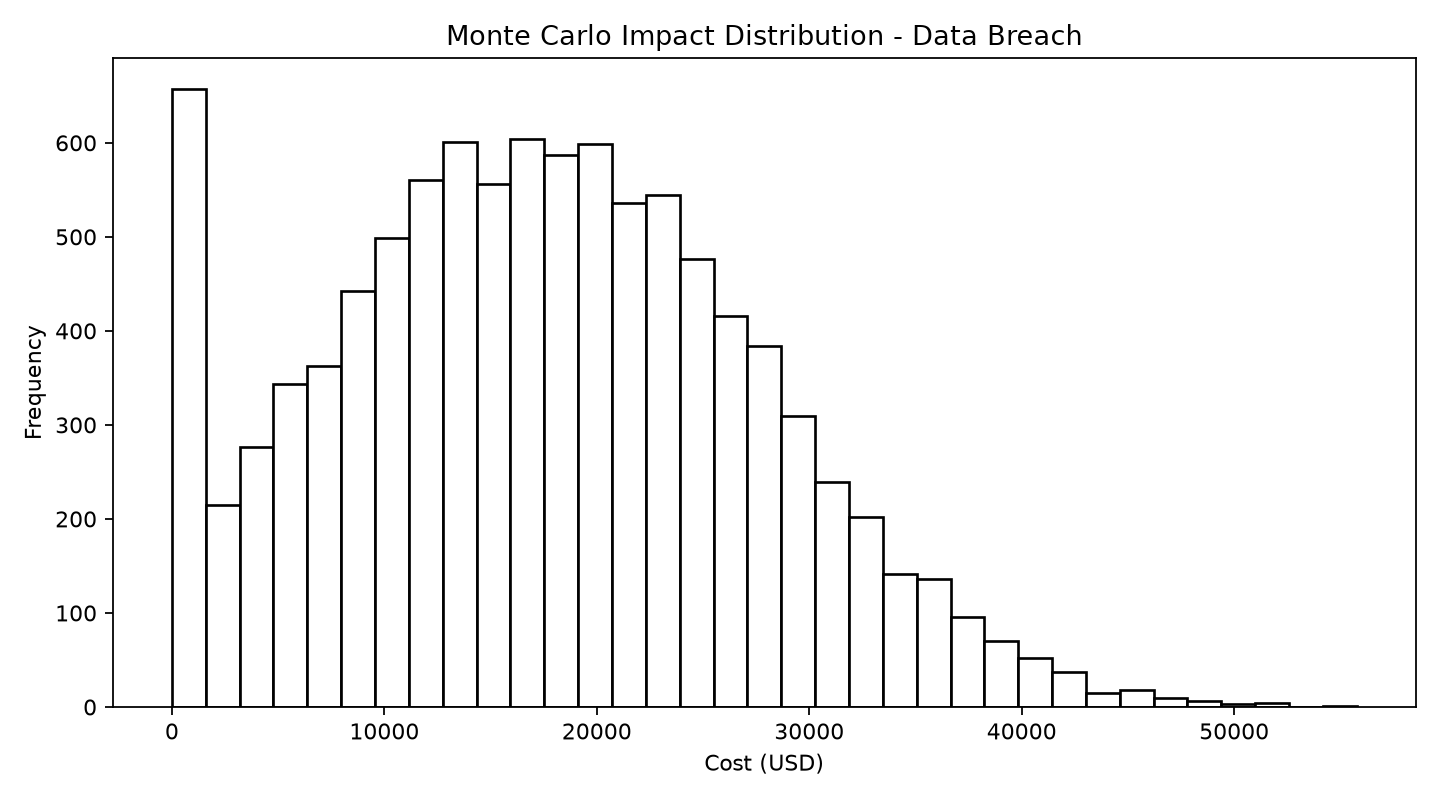
\includegraphics[width=\linewidth]{figures/histogram_dataBreach_impact.png}}}
  \caption{We ran a\index{Monte Carlo simulation} Monte Carlo simulation of 10,000 iterations with a normal distribution to spread random instances between bounds taken from means of seven year samples. We set a lower bound that the events would cost at \$0.  We set an upper bound that the events would cost \$33{,}527.27.  \protect\endnote{\index{sample} Sample size was set equivalent to the City of\index{Chattanooga} Chattanooga to determine the per capita rates for each year over data from \index{American Samoa} American Samoa and\index{California} California.  The means of those rates were used to set upper and lower bounds with \index{American Samoa} American Samoa and\index{California} California representing low and high \index{cybercrime} cybercrime impact values respectively.}
  \protect\endnote{Monte Carlo Modeling Toolkit authored by Derek E. Brink, CISSP, \url{www.linkedin.com/in/derekbrink}. March 2023.}
  }
  \label{fig:screenshot-montecarlo-databreach-impact-histo}
\end{figure}
\begin{figure}[H]
  \centering
  \rotatebox{0}{\scalebox{1}{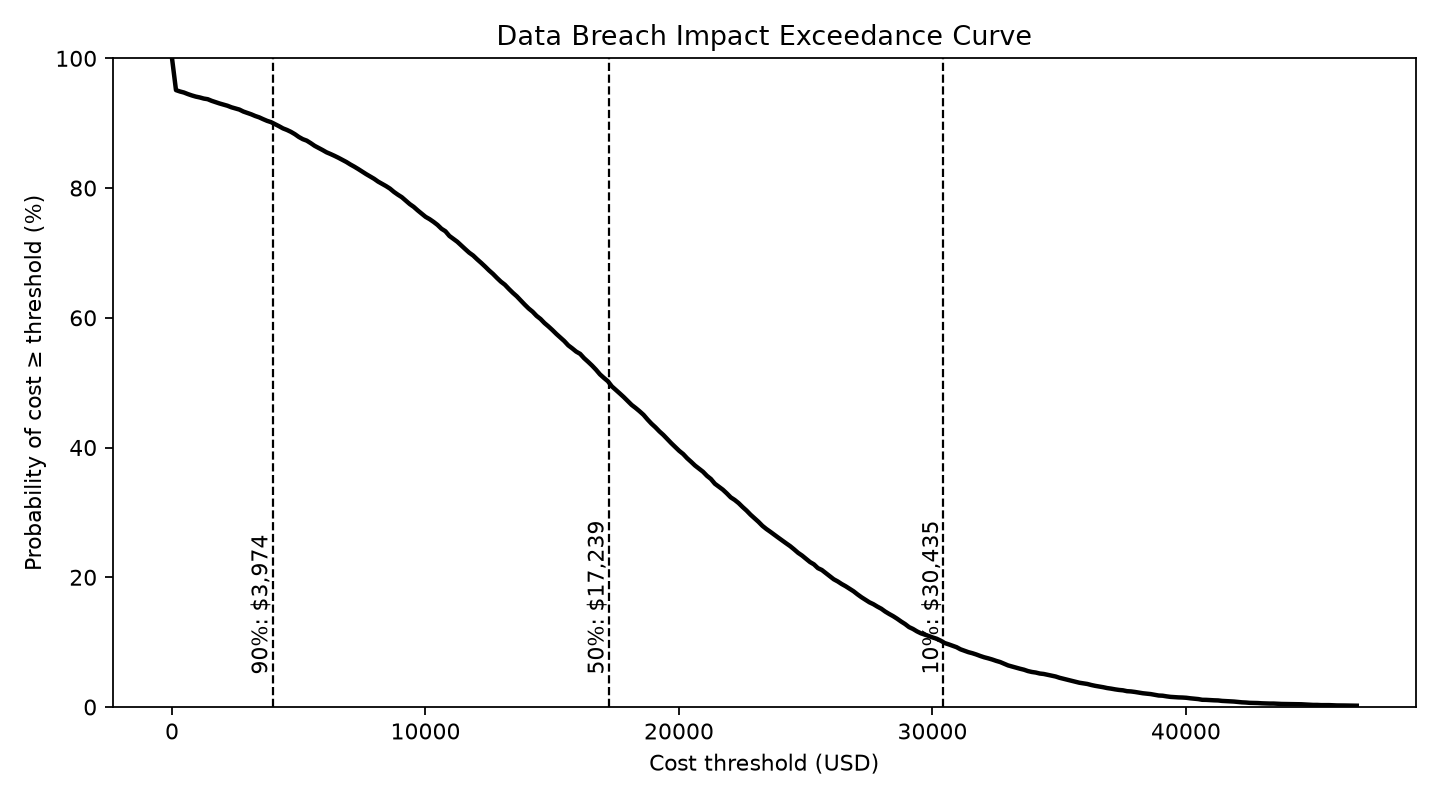
\includegraphics[width=\linewidth]{figures/percent_dataBreach_impact.png}}}
  \[
\mathrm{CI}_{80\%}(\theta) = [\$3{,}824, \$30{,}365]
\]
  \caption{A\index{Monte Carlo simulation} Monte Carlo simulation with a normal distribution suggests that there is a 90\% probability that\index{data breach} data breach events will cost \$3{,}824 or more in a year.  There is a 50\% likelihood that they will cost \$17{,}120 or more in a year.  There is a 10\% chance that they will cost \$30{,}365 or more in a year. \protect\endnote{\index{sample} sample size was set equivalent to the City of\index{Chattanooga} Chattanooga to determine the per capita rates for each year over data from \index{American Samoa} American Samoa and\index{California} California.  The means of those rates were used to set 10\% and 90\%\index{confidence interval} confidence intervals with \index{American Samoa} American Samoa and\index{California} California representing low and high \index{cybercrime} cybercrime impact values respectively.}
  \protect\endnote{Monte Carlo Modeling Toolkit authored by Derek E. Brink, CISSP, \url{www.linkedin.com/in/derekbrink}. March 2023.}
  }
  \label{fig:screenshot-montecarlo-databreach-impact-percent}
\end{figure}
